\section*{Appendix A. Worked Examples}
\addcontentsline{toc}{section}{Appendix A. Worked Examples}

\footnotesize
\noindent\textbf{Hinglish, English question, wrong.} Date subtraction, short. ``Today is 2025-05-01, what was the date 3 days ago?'' Gold 2025-04-28. Standard English CoT answered correctly. Excerpt: \emph{Step 4: 01 minus 3 karne par hum 31 April par aayenge. Step 5: Isliye, 3 days ago ki date 2025-04-30 thi.} Answer: 2025-04-30.

\smallskip
\noindent\textbf{en-CoT, $k=1$, backward answer.} Date recurrence, short, ID 5, time-related distractor, Hindi question with \hi{आज को छोड़कर, 1वीं आवृत्ति}. Excerpt: \emph{Given the phrasing ``excluding today,'' this suggests we need to find what comes before.} Answer: 2025-04-06. Gold 2025-04-14.

\smallskip
\noindent\textbf{CLP, stage 1 anchors stage 2.} Date recurrence, long, ID 12, no distractor. Stage 1 ends: \emph{Therefore, the date of the 7th occurrence is 2 August 2027.} Stage 2 ends: \emph{Adding 78 days to 16 May 2027 also results in 2 August 2027.} Answer: 2027-08-02. Gold 2027-08-15.

\smallskip
\noindent\textbf{Resampling arms.} Date recurrence, long, ID 12, Hindi, time-related distractor. The original trace answered 2027-04-20. Correct continuations out of seven: Q 5, P 2, M 0, P1 2. A single example cannot show an effect; Figure~\ref{fig:interventions} gives the aggregates.

\normalsize
\section*{Appendix B. Secondary Figures}
\addcontentsline{toc}{section}{Appendix B. Secondary Figures}

\begin{figure}[!ht]
\centering
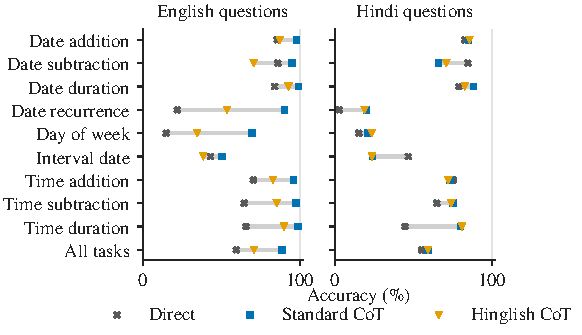
\includegraphics[width=\columnwidth]{hinglish_tasks}
\caption{Accuracy by task under the Hinglish prompt, answered.}
\label{fig:hingtasks}
\end{figure}

\begin{figure}[!ht]
\centering
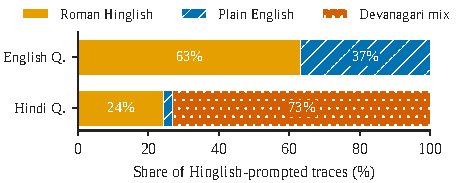
\includegraphics[width=\columnwidth]{hinglish_style}
\caption{Script style of Hinglish-prompted traces.}
\label{fig:hingstyle}
\end{figure}

\begin{figure}[!ht]
\centering
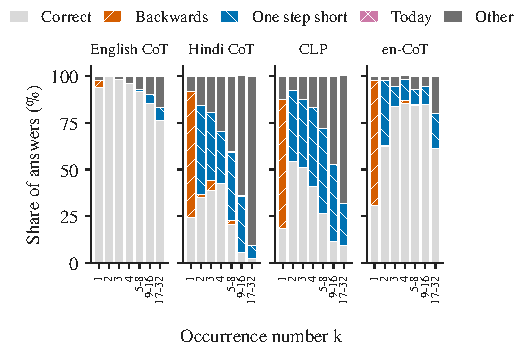
\includegraphics[width=\columnwidth]{recurrence_k}
\caption{Date recurrence answers by occurrence number $k$, on 2,250 questions. Backward answers concentrate at $k=1$ under every prompt on Hindi questions; one-step-short answers run through every $k$.}
\label{fig:recurrence}
\end{figure}

\begin{figure}[!ht]
\centering
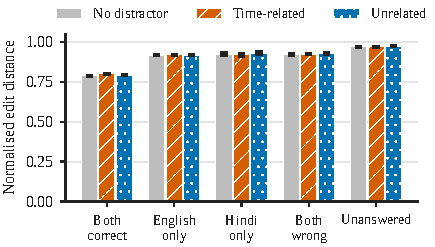
\includegraphics[width=\columnwidth]{ed_outcome}
\caption{Mean RDS by correctness outcome and distractor condition. Failure outcomes sit about 0.13 above both-correct.}
\label{fig:edoutcome}
\end{figure}

\begin{figure}[!ht]
\centering
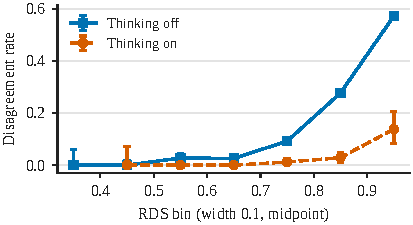
\includegraphics[width=\columnwidth]{lr_bins}
\caption{Observed disagreement rate by RDS bin. Answer tokens are included, so this rise is largely mechanical.}
\label{fig:lrbins}
\end{figure}

\begin{figure*}[t]
\centering
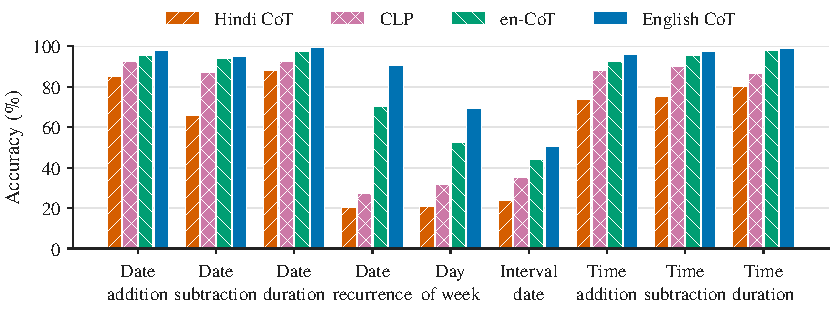
\includegraphics[width=0.92\textwidth]{task_bars}
\caption{Answered accuracy by task on 2,250 questions.}
\label{fig:taskbars}
\end{figure*}

\begin{figure*}[t]
\centering
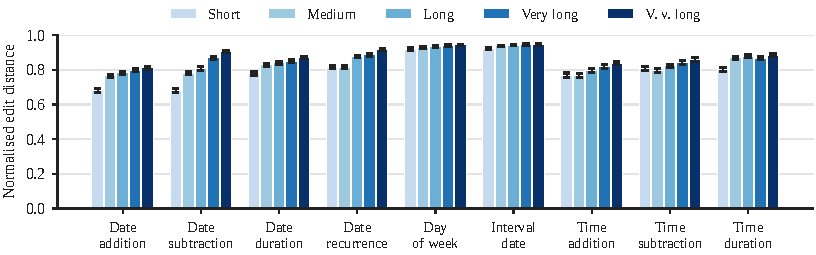
\includegraphics[width=0.92\textwidth]{ed_task_difficulty}
\caption{Mean RDS by task and difficulty, standard and thinking-on visible replies pooled, error bars treating pairs as independent. Means sit near the ceiling on day of week and interval date, so RDS cannot track difficulty there.}
\label{fig:edtask}
\end{figure*}
